\chapter{Life of a Coronal Bright Point\\ and its Filament Channel}\label{Chap:cbps}


Here we investigate how photospheric flows cause changes in the chromosphere and corona, specifically prominence stability and coronal bright point (CBP) evolution. This is done through the exploration of the manifestation of a coronal bright point where a filament is known to form in, and erupt from, its associated polarity inversion line. We focus on a flux emergence event and how its relationship with photospheric flows affect the formation of CBPs and the stability of associated filaments. We also investigate the notion that flux emergence originates in the centre of a supergranular cell and migrates towards the supergranular network on the outskirts of the cell. Two minifilament eruptions are observed during the CBP observation, implying that the filament only partially erupts, or fully erupts and the filament channel refills with plasma prior to the second eruption. 

\section{Coronal Bright Points}
\label{cbp}
Coronal bright points (CBPs) consist of low, small scale, coronal loops with enhanced coronal emission in the EUV and X-ray. These loops trace out the connection between flux patches of opposite polarity in the solar photosphere. They are found all over the solar disc in active regions, coronal holes, and quiet Sun. The CBP discussed here is found in a coronal hole. CBPs are linked to transient phenomena such as jets, mass ejections and `minifilament' production \citep{sterling_small-scale_2015,sterling_minifilament_2016}. In X-rays they are seen to have a diameter of 20$''$ to 30$''$ (15~Mm to 22~Mm) with a bright core of 5$''$ to 10$''$ (4~Mm to 7~Mm) \citep{madjarska_coronal_2019}; in Extreme Ultraviolet (EUV), \cite{zhang_spatial_2001} report an average size of $14''\times14''$ (10~Mm$\times$10~Mm). Recently, using the Extreme Ultraviolet Imager \citep[EUI;][]{rochus_solar_2020} aboard Solar Orbiter \citep[SolO; ][]{muller_solar_2020}, \cite{berghmans_extreme-uv_2021} observed small scale coronal brightenings dubbed `solar campfires'. These campfires are thought to be fine scale heating events in the solar corona. \cite{panesar_magnetic_2021} suggests that some of these solar campfires may be CBPs. This would suggest that some CBPs could be as small as $1''\times1''$ (725~km$\times$725~km).


Considering their plasma properties, it can be surmised that they are essentially downscaled active regions (ARs). The loops which make up CBPs range from temperatures of 1.2 to even as high as 3.4~MK. Their electron densities also vary from $10^9$~cm$^{-3}$ at transition region temperatures to $10^8$~cm$^{-3}$ at coronal temperatures \citep{madjarska_coronal_2019}. A study of ARs by \cite{del_zanna_solar_2003} using the Transition Region and Coronal Explorer \citep[TRACE;][]{handy_transition_1999}; and the Coronal Diagnostic Spectrometer \cite[CDS;][]{harrison_coronal_1995} onboard the Solar and Heliospheric Observatory \citep[SOHO;][]{domingo_soho_1995} found temperatures of 0.7 to 1.1~MK and electron densities of $10^8$~cm$^{-3}$ to $10^9$~cm$^{-3}$ in loops in an AR which are of a similar order of magnitude to CBPs. 

CBPs have a large range of lifetimes, however, their mean lifetime was found to be 8 hours by a statistical study of Skylab X-ray CBPs by \cite{golub_solar_1974}. Considering the mean solar rotation rate of 27.27 days \citep{stenflo_time_1990} this allows a unique opportunity to investigate the properties of CBPs over their entire lifetime without rotating out of view. Their occurrence appears to be anti-correlated with the solar cycle, with more appearing during solar minimum than solar maximum \citep{davis_solar_1977}. A study by \cite{nakakubo_variation_2000} with the Soft X-ray Telescope \citep[SXT;][]{tsuneta_soft_1991} aboard the Yohkoh \citep{ogawara_solar-mission_1991} spacecraft suggest that this increase near solar minimum is due to a decrease in background intensity, which allows for fainter CBPs to be detected. The follow-up study \citep{hara_variation_2003} showed that this anti-correlation between CBP number and sunspot number was clearly evident in dark areas (such as coronal holes); but in bright areas they are correlated with sunspot number.


\section{Supergranules}
Solar granules are small convective cells on the order of $1.4''$ (1~Mm) in size and pave the solar surface \citep{nordlund_solar_2009}. They convect heat from the solar interior and deposit it in the photosphere and higher. These granules form larger structures named supergranules, whose global behaviour is similar to that of the local behaviours of granules. The discovery of supergranules by \cite{hart_motions_1956} led to the first measurement of the 15-minute oscillations on the Sun which gave rise to the birth of the field of helioseismology.
Supergranules have horizontal scales of roughly 25$''$ to 70$''$ (20~Mm to 50~Mm) and if we assume that granules are simply advected by the plasma flow inside their parent supergranules, their horizontal internal motions can be tracked using methods such as Local Correlation Tracking \citep[LCT;][]{november_precise_1988,rincon_suns_2018}. Here we use Fourier Local Correlation Tracking (FLCT; see section \ref{flct}) . 
Flows within supergranules are observed to appear at their centre and flow outwards towards the boundary with other supergranules \citep[e.g.][]{muglach_photospheric_2021}. This sort of motion is consistent with the classic view of convective heating.
With the appropriate scaling of the flow vectors, the supergranular network can be outlined by simply plotting their flow vectors (see left of Fig. \ref{supergrans} as an example).
\begin{figure} 
    \centering
    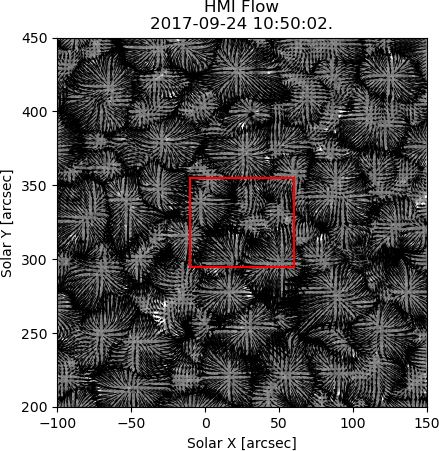
\includegraphics[width=0.435\linewidth]{./04CBPs/figs/grans.png}
    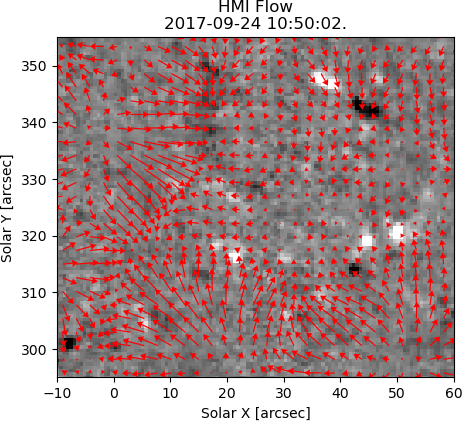
\includegraphics[width=0.49\linewidth]{./04CBPs/figs/smallflow.png}
    \caption[Supergranular flows and Zoomed Window of Region of Interest.]{\textit{left}: Supergranules outlined by their flow vectors and box outlining the smaller considered region. \textit{right}: The smaller region to be considered in analyses (arrows here are red for better contrast). The flow field here is averaged over one hour and the time of the background images are the middle of this hour.}
    \label{supergrans}
\end{figure}


\section{Observations and Preprocessing}


The data used in this study come from the 193~\AA{} and 304~\AA{} filters from the Atmospheric Imaging Assembly \citep[AIA; ][]{lemen_atmospheric_2012}, and the Helioseismic Imager \citep[HMI; ][]{scherrer_helioseismic_2012} instruments onboard the Solar Dynamics Observatory \citep[SDO; ][]{pesnell_solar_2012}.

The HMI and AIA data were downloaded from the Virtual Solar Observatory (VSO) repository via the SolarSoftware (SSW) IDL routines \comp{vso\_search} and \comp{vso\_get}. Additionally, the data was taken to level 1.5 using \comp{aia\_prep}. Next the effects of solar rotation were removed by `rotating' the images to a common time through the use of IDL mapping software. The FOV was then reduced to encapsulate only the CBP \footnote{This data was prepared by Drs. K. Muglach and A. Leisner. The processed datacubes were provided to A. W. Peat for analysis.}.

\subsection{Timeline}
On the 25th September 2017 at approximately 00:05~UTC a flux emergence was observed in a coronal hole in the north of the Sun (see \fig{fig:setup} for the location of this coronal hole). This flux emergence soon created a CBP, with the event 
\begin{figure}
    \centering
    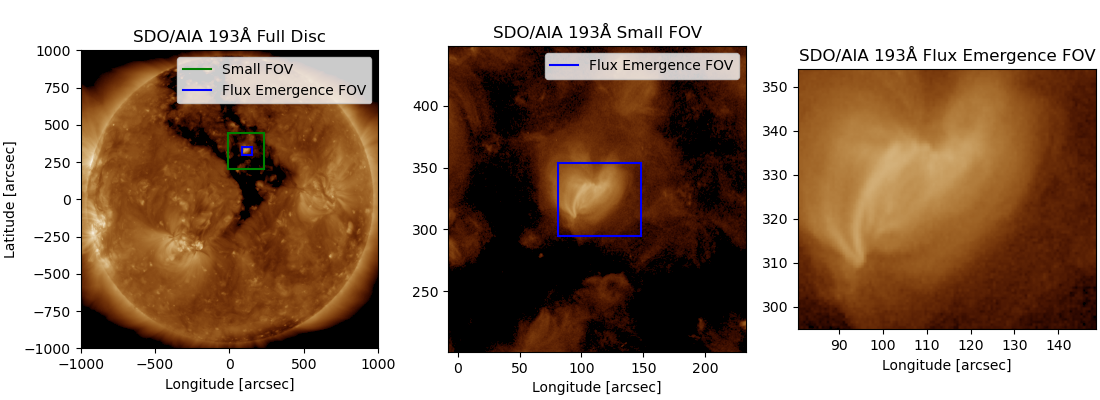
\includegraphics[width=\linewidth]{./04CBPs/figs/193context.png}
    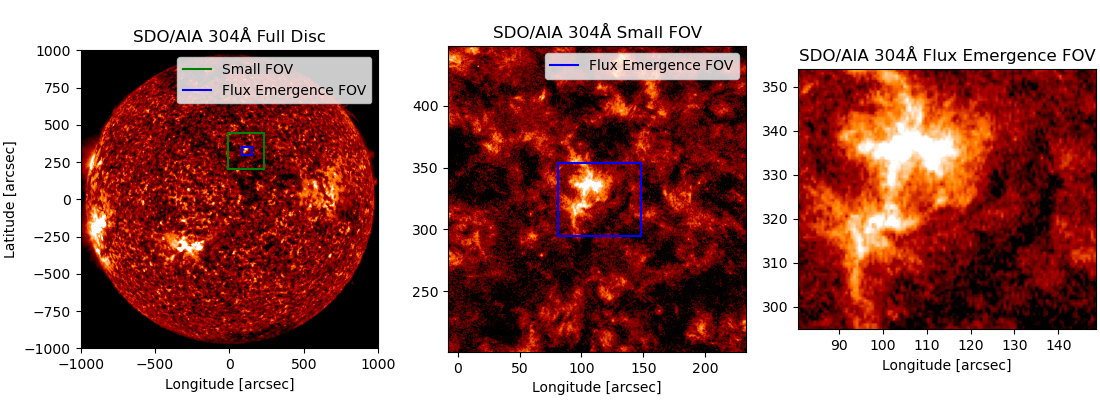
\includegraphics[width=\linewidth]{./04CBPs/figs/304context.png}
    \caption[Location of the Coronal Bright Point in 193~\AA{} and 304~\AA.]{Location of the Coronal Bright Point in 193~\AA{} and 304~\AA{}. The filament is not easily seen in these channels.}
    \label{fig:setup}
\end{figure} %this line break works, so I'm not touching this
peaking at approximately 10:00, and ended on the 27th September 2017 at approximately 12:45. The timeline of this event can be seen in figure \ref{fig:cbptl}; on the bottom panel, the dash-dot lines represent midnight, and the dashed line corresponds to the time at which the top panels were taken. A brief summary of this timeline is as follows; on 2017-09-24, at 23:55, the flux emergence begins. On 2017-09-25, at 00:05, bright loops begin to form in the EUV channels - 193~\AA\ and 304~\AA. At 01:25 a dark core becomes visible in 304~\AA. At 01:40, the emerged magnetic patches are fully formed. At 04:40 the dark core seen in 304~\AA\ is no longer visible, possibly obscured by the overlying brighter material. At 09:50, the peak intensity of the event is reached in both the 193~\AA{} and 304~\AA{} filters. At 16:50, the two emerged fluxes are at their maximum distance from one another. At 17:00 the negative patches begin to fracture and cancel out with solitary positive patches. At 21:10, the emission in 304~\AA\ and 193~\AA\ begins to greatly reduce. By 22:40, the negative flux patch has fragmented into many smaller patches. The CBP then gradually decays, ending on 2017-09-27 at 12:45.

\begin{figure}
    \centering
    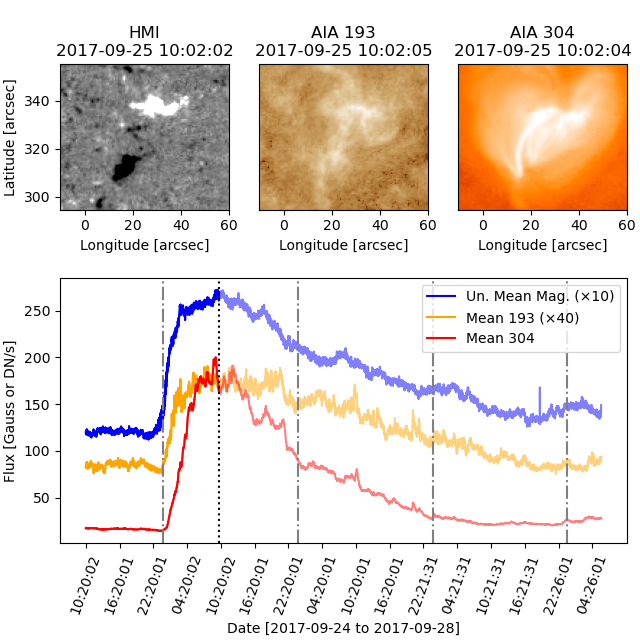
\includegraphics[width=\linewidth]{./04CBPs/figs/1896.png}
    \caption[Timeline of Flux Emergence]{\textit{Top left}: HMI magnetogram of the flux emergence; \textit{Top middle}: AIA 193~\AA\ view of coronal bright point; \textit{Top right}: AIA 304~\AA\ view of flux emergence. \textit{Bottom}: Timeline of the CBP and flux emergence. The dotted line represents the time at which the top panels were taken. The dash-dot lines represent midnight.}
    \label{fig:cbptl}
\end{figure}

In order to use Fourier Local Correlation Tracking (FLCT; see section \ref{flct}) on the HMI intensity observations, solar p-mode oscillations \citep{deubner_observations_1975} must be removed from the data otherwise FLCT may interpret these oscillations as movement across the solar surface. To remove these p-mode oscillations, the HMI intensity images were first converted into a datacube, introducing a third dimension, time. The Fourier transform of this datacube was then taken. These frequencies recovered by the Fourier transform were converted to velocities by including the spatial scale of the images. Oscillations of less than some threshold velocity were removed before Fourier transforming back into a time series. For this threshold velocity, integer values in the range 0 to 5~km~s$^{-1}$ were tested. A value of 3km~s$^{-1}$ was determined to be the ideal value. Velocities of 4 and 5~km~s$^{-1}$ did not show any appreciable change in the time series when compared with that of 3~km~s$^{-1}$. 

\section{Fourier Local Correlation Tracking}
\label{flct}
Fourier Local Correlation Tracking \citep[FLCT;][]{welsch_ilct_2004,fisher_flct_2008} was employed to track the motions of the HMI intensity images. Here, FLCT is implemented through \comp{pyflct} version 0.2.2 by the SunPy Project \citep{barnes_sunpy_2020}. FLCT takes five mandatory inputs; the two images, their temporal difference, their spatial resolution, and sigma. Sigma is the standard deviation of the Gaussian which the images are multiplied by later in the algorithm. This is required to calculate the local correlation. If this number is too small, it may not encapsulate the movement of the feature; if it is too large, it may smooth out the smaller velocities. It is imperative to find sigma such that you are able to track the largest expected velocities, but not smooth out the smaller scale movements. Both images are multiplied by this Gaussian centred on the currently considered pixel. This is done on a pixel by pixel basis and is not a convolution over the whole image, each pixel is considered separately. Areas where the Gaussian-multiplied image goes below some threshold (0.01 by default) are discarded from the calculation for that pixel in order to expedite the method. A custom threshold value may be set to skip calculations of pixels below the threshold, further expediting the algorithm. The two considered succesive frames are then cross correlated and the cross correlation results are cubic interpolated to find the maximum of the cross correlation to sub pixel precision. Then, in combination with the temporal difference, the velocities can be determined. This is then repeated for every pixel. Increasing sigma results in an increase in computation time, therefore it is important to find a compromise which reduces computation time while producing a meaningful result. Integer values in the range 5 to 20 were tested as values of $\sigma$ on the entire data set. It was found that $\sigma\approx10$ or higher produced similar results, and so a value of 12 was chosen. This cautiously overestimates the maximum expected distance for a feature to move in order to ensure the validity of the results. The resulting flows recovered by FLCT were then averaged over 1 hour of observations to remove any erroneous vectors. Each of these new flows were separated by 30 minutes to give some overlap into the previous one hour window and to give a better representation of the flow.

\section{Results and Discussion}
\label{fluxing}
With the flow fields from FLCT, the boundaries of the supergranules were easily revealed (see left of Fig. \ref{supergrans}). However, here we focus on a smaller region (right of Fig. \ref{supergrans}, and Fig. \ref{fig:setup}) in the spatial ranges $x\in[-10, 60]$ and $y\in[295, 355]$ arcseconds respectively. As based on HMI magnetograms, this is where the bright point is anchored.
\begin{figure}
    \centering
    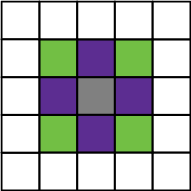
\includegraphics[width=0.3\linewidth]{./04CBPs/figs/connectvitity.png}
    \caption[Graphical Representation of Connectivity]{Connectivity. The considered pixel here is in grey. The purple pixels are considered 1-connected, and the green are considered 2-connected. This connectivity is named such as it states how many orthogonal lateral hops are required to reach that pixel from the considered pixel.}
    \label{fig:connect}
\end{figure}
Additionally, the relationship between the motions derived from HMI intensity images and magnetic patches in the co-temporal magnetograms could be investigated. A magnetic patch is defined as any group of contiguous (at most 2-connected) pixels with a magnetic flux magnitude of 30~G or more (see figure \ref{fig:connect} for a visual representation of connectivity). It is also possible for a single pixel to be in a patch by itself. The velocity vectors of all the co-spatial intensity and magnetic patch pixels were summed to make a total velocity vector for the patches. It is assumed that all pixels within the same magnetic patch are globally co-moving. 

\begin{figure}
    \centering
    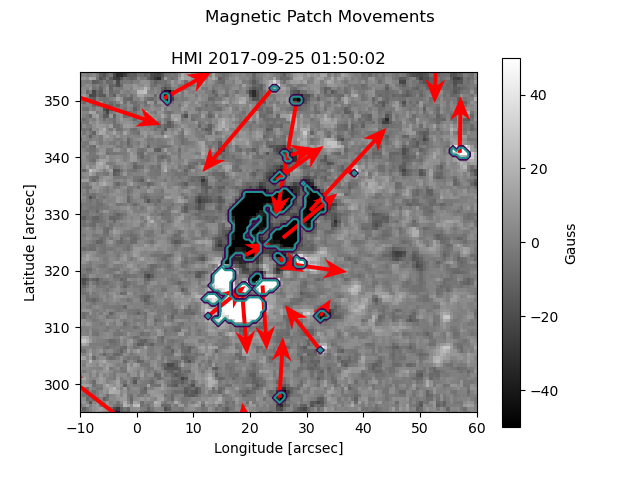
\includegraphics[width=0.49\linewidth]{./04CBPs/figs/030.png}
    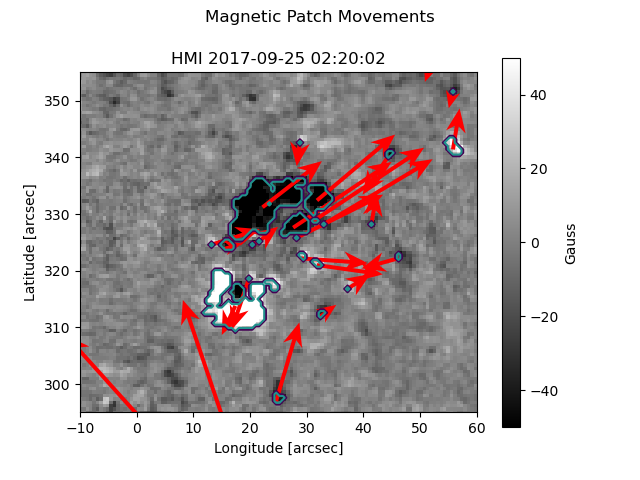
\includegraphics[width=0.49\linewidth]{./04CBPs/figs/031.png}
    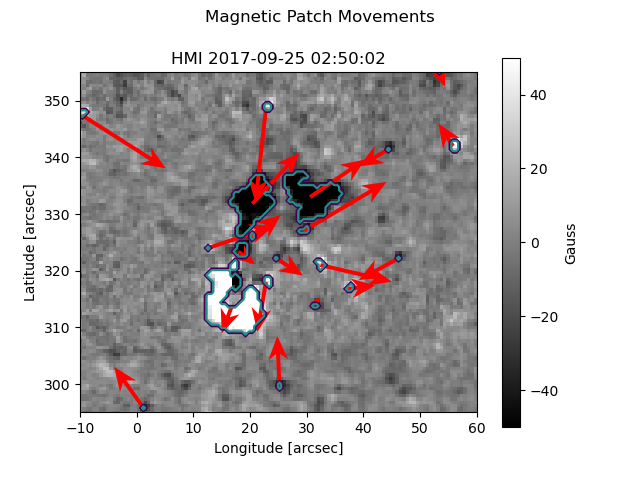
\includegraphics[width=0.49\linewidth]{./04CBPs/figs/032.png}
    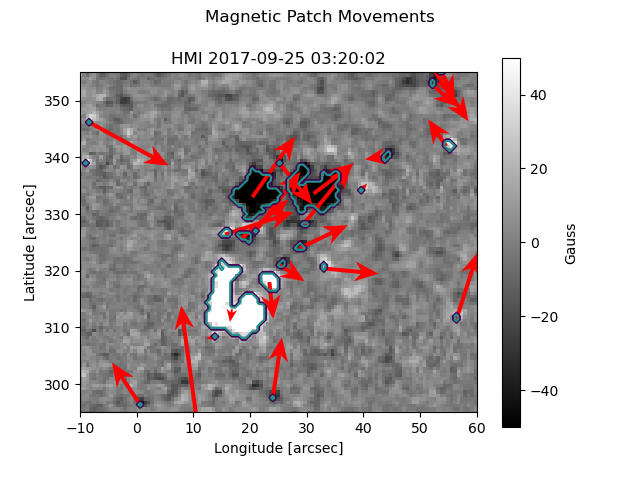
\includegraphics[width=0.49\linewidth]{./04CBPs/figs/033.png}
    \caption[Global Movement of 2-connected Magnetic Patches]{Movement of magnetic patches. 2-connected patches, above a magnetic flux magnitude of 30G, are outlined in cyan with their mean vectors drawn in red. These magnetic flux images have been set to saturate at $\pm50$~G. The length of the arrows here are not to scale and are exaggerated for clarity.}
    \label{fig:single_patchlabels}
\end{figure}

From figure \ref{fig:single_patchlabels}, it is evident that the magnetic patches move according to the velocity vectors found by FLCT from the HMI intensity images. It can then be concluded that movements in the photosphere influence the migration of magnetic patches. This will then affect the life and evolution of any solar filament located here. \cite{roudier_horizontal_2018} and \cite{wollmann_evolution_2020} showed that horizontal flows in the photosphere can lead to filament eruptions. Therefore, following that work, we can say that these filament eruptions might occur for the same reason. However, we wish additionally propose as the flux emergence continues and begins to disappear, this leads to the reconfiguration of the polarity inversion line resulting in minifilament eruptions. The smaller patches that seem to appear and disappear between frames are areas that simply just rise above or fall below the magnetic threshold. Their transient nature gives little credence to the flow vectors attached to them. These flow vectors do indeed show the flow of the HMI magnetograph images, but do not necessarily show where these small transient patches will move to.

Additionally, the flux emergence seems to appear at the boundary of two supergranules. The positive patch mostly remains at the boundary where it formed, but the negative patch is pulled up by flows of the interior of the cell where it remains from approximately 06:20 to 16:50 on 2017-09-25. It then continues to coast along the boundary of two cells where it is slowly torn apart and cancelled by other positive patches on the Sun, having mostly disappeared by 17:20 on 2017-09-26.

%\section{Discussion}

With flux emergence like this inevitably comes a polarity inversion line where a filament may form. Two minifilament eruptions were observed over the length of the observation suggesting the formation of at least one filament channel which either refilled and erupted a second time, or partially erupted and then partially or fully erupted later. The two minifilament eruptions occur on 2017-09-26 at 10:10 and 16:15~UTC. These eruptions are accompanied by small brightenings seen in 193~\AA\ and 304~\AA\ in Figs \ref{fig:cbptl} and \ref{fil1}. 

For the first eruption, seen at 10:10~UTC, the mechanism leading to the partial eruption appears to be a reconfiguration of the field as the negative polarity to the North-West of the image combines with a smaller patch. This affects the polarity inversion line which in turn affects the stability of the filament leading to a partial eruption.
\begin{figure}
    \centering
    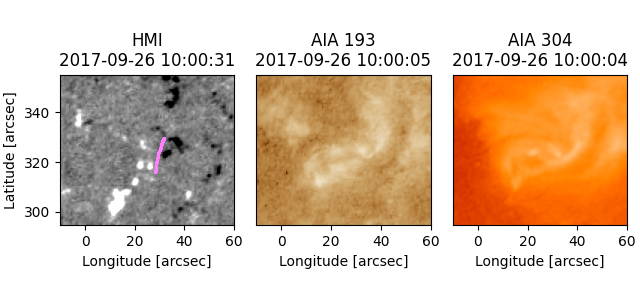
\includegraphics[width=.8\linewidth]{./04CBPs/figs/before1.png}
    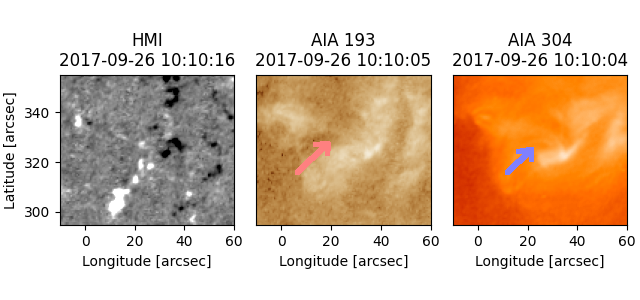
\includegraphics[width=.8\linewidth]{./04CBPs/figs/during1_overlay.png}
    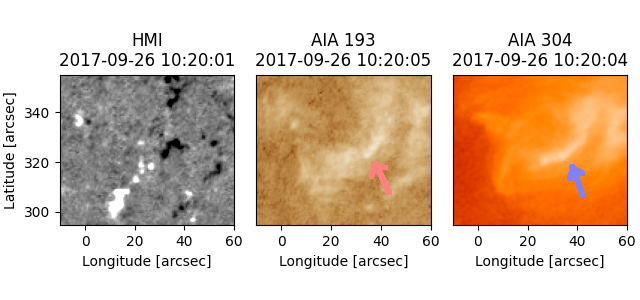
\includegraphics[width=.8\linewidth]{./04CBPs/figs/after1_overlay.png}
    \caption[The first minifilament eruption.]{The first minifilament eruption. \textit{Top}: 10 minutes prior to the eruption. The magenta line shows the approximate location of the polarity inversion line. \textit{Middle}: During the eruption. The arrows indicate the erupting material. \textit{Bottom}: 10 minutes post the eruption. The arrows indicate the brightenings in the magnetic footpoints from heated material now emitting in the coronal AIA filters.}
    \label{fil1}
\end{figure}
There is also a second eruption approximately 4 hours later at 16:15~UTC. Contrary to the first eruption, this filament eruption is caused by flux cancellation removing the polarity inversion line entirely. The field lines are believed to have been tangled in a complex manner which, upon reconnection, caused the filament channel to erupt.  Figs. \ref{fig:cbptl} and \ref{fil2} shows the stages of the eruptions. Admittedly, both eruptions are hard to see in still images, and are much clearer in movies of the event.
\begin{figure}
    \centering
    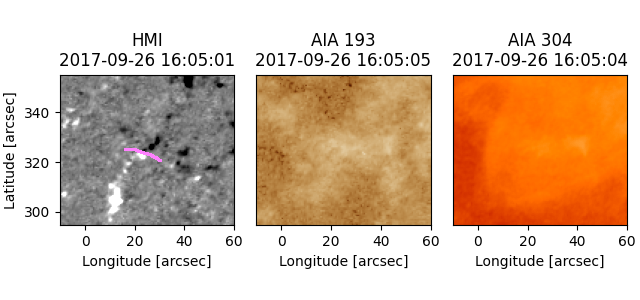
\includegraphics[width=.8\linewidth]{./04CBPs/figs/before2.png}
    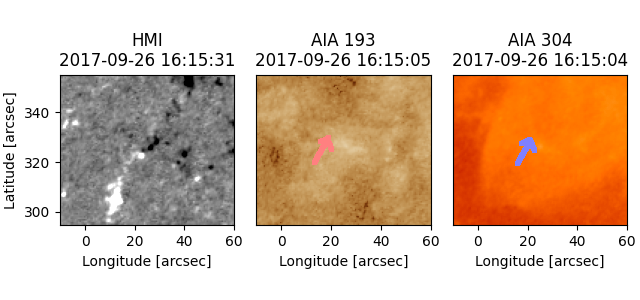
\includegraphics[width=.8\linewidth]{./04CBPs/figs/during2_overlay.png}
    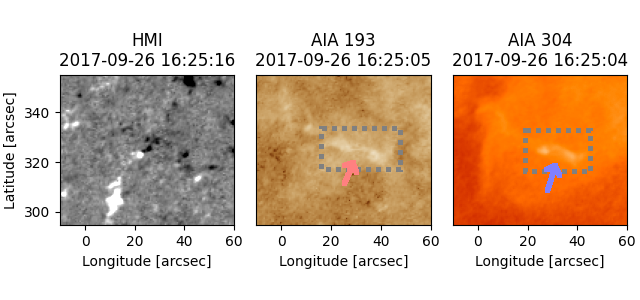
\includegraphics[width=.8\linewidth]{./04CBPs/figs/after2_overlay.png}
    \caption[The second minifilament eruption.]{The second minifilament eruption. \textit{Top}: 10 minutes prior to the eruption. The magenta line shows the approximate location of the polarity inversion line. \textit{Middle}: During the eruption. The arrows indicate the erupting material. \textit{Bottom}: 10 minutes post the eruption. The footpoints are brightened post-eruption, the location of these are indicated by the arrows and dotted box. The photospheric magnetic footpoints here move towards each other and begin to perform flux cancellation within the region of the dotted box.}
    \label{fil2}
\end{figure}
With these results we can better understand how the photospheric magnetic flux determines the evolution of the filaments and CBPs.


\section{Concluding Remarks}
It is evident that photospheric flows do indeed influence the migration of magnetic patches across the solar disc. However, here we were able to isolate independent magnetic patches and track their global movement from the mean flow vectors of their constituent pixels. Compared to previous studies such as \cite{roudier_horizontal_2018} and \cite{muglach_photospheric_2021}, as opposed to evaluating the behaviour of the photospheric flows on a global scale, we are able to assign flow vectors to individual patches of magnetic flux. This allows us to tie the behaviour of the minifilaments and the CBPs to the magnetic flux patches as opposed to the movement of the photosphere. The two minifilament eruptions appear to be caused by two different mechanisms. The former from a reconfiguration of the magnetic field and therefore PIL, and the latter due to the annihilation of the PIL through flux cancellation of the patches that bound the line. Future work could be done on isolated erupting filament structures such that we can study the effects of migrating patches of magnetic flux pertinent only to the filament in greater detail without interference from other magnetic structures in the vicinity. However, given the long lifetime of such isolated/quiescent filaments, it may prove difficult to find a suitable candidate for such analyses.